\chapter{Space-Time Ambiguity Function}
\label{chapter:stamb}
\thispagestyle{myheadings}

% set this to the location of the figures for this chapter. it may
% also want to be ../Figures/2_Body/ or something. make sure that
% it has a trailing directory separator (i.e., '/')!
\graphicspath{{3_STAmb/Figures/}}

%%%%%%%%%%%%%% Intro %%%%%%%%%%%%%%%%%%%%%%%%%%%%%%%%%%%%%
This chapter explains the theoretical backbone for sampling issues associated with ISR. The first section will detail the differences in space-time sampling between single antenna and electronically steerable array (ESA) systems. The next section will then detail the derivation of the space-time ambiguity. Lastly the impact of moving plasma on the apparent ambiguity will be shown, both from a theoretical stand point and a demonstration using collected ISR data.


\section{Space-Time Sampling}
\label{sec:sptimesamp}
These new ESA based systems differentiate themselves from dish antennas in a fundamental way. Instead of dwelling in a single beam or scanning along a prescribed direction, an ESA can move to a different beam position within its field of view on a rapid, pulse by pulse basis. An illustration of the differences between ESA and conventional radar systems with respect to statistical integration of radar pulses, focusing on time history of beam positions, starts with the desired grid of geographic parameter coverage in Figure \ref{fig:bp1}. Figure \ref{fig:dbsts} shows a possible path for a dish based antenna to cover this measurement space through moves to different beam positions through time, represented on the z-axis as pulse repetition intervals (PRIs). The dish sweeps through the field of view in a continuous scan.  In contrast, an ESA system can instead move from position to position in discrete steps as seen in Figure \ref{fig:phbsts}. It is noted as well that the phased array antenna is able to collect data from different beams during overlapping time periods, creating a lattice like pattern. This type of pulse-to-pulse beam position change is very difficult to accomplish with dish antenna systems having significant pointing inertia. 

\begin{figure}
	\centering
	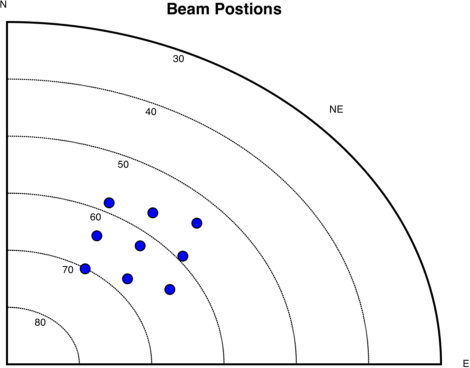
\includegraphics[width=3.5in]{beampositionssts}
	\caption{A 3x3 grid of desired measurement positions in a
         hypothetical geodetic latitude/longitude space. }
	\label{fig:bp1}
\end{figure}

\begin{figure}
	\centering
	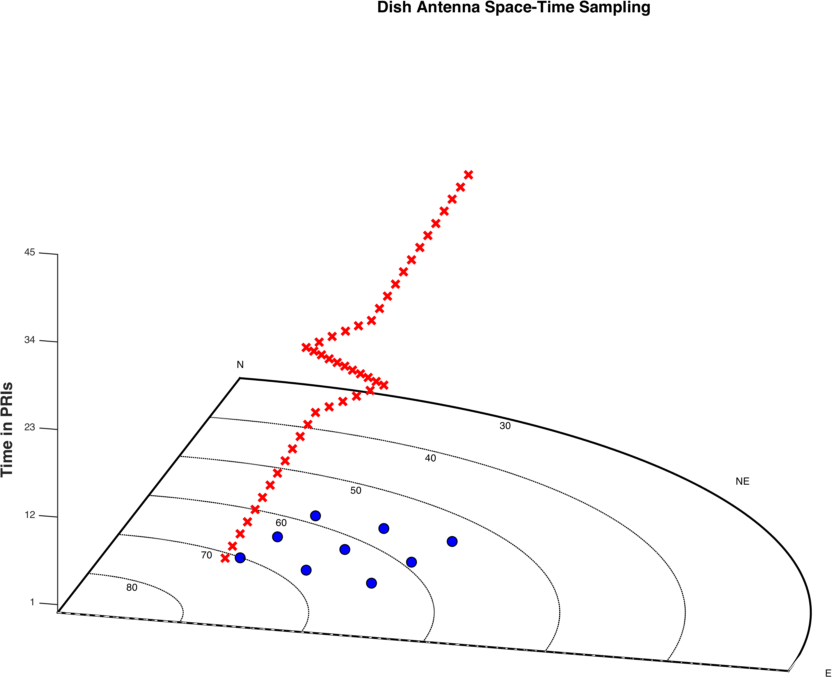
\includegraphics[width=3.5in]{dishsts}
	\caption{Space-time sampling of the measurement space from Figure~\ref{fig:bp1} using a dish based antenna, where the red x's mark the pulse in beam space and time. Beam positions from Figure \ref{fig:bp1} are shown below in blue at $z=0$.}	
	\label{fig:dbsts}
\end{figure}

\begin{figure}
	\centering
	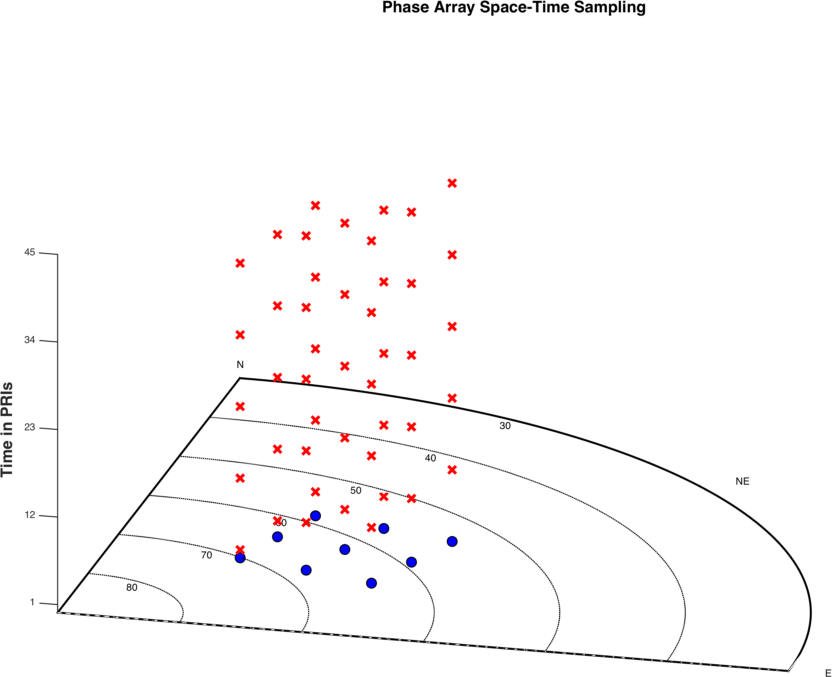
\includegraphics[width=3.5in]{phasedarraysts}
	\caption{Space-time sampling of the measurement space from Figure~\ref{fig:bp1} using a phased array based antenna, where the red x's mark the pulse in beam space and time. Beam positions from Figure \ref{fig:bp1} are shown below in blue at $z=0$.}	
	\label{fig:phbsts}
\end{figure}

The rapid steering ability of ESA systems relative to space-time sampling yields a new flexibility, in post processing, to statistically combine information from different beams using knowledge of the plasma velocity field, where this information is obtained either from external sources or from the Doppler shift of the ionospheric echoes themselves. This can help to relax the assumption of stationarity for plasmas that are evolving or changing their shape on time scales longer than the integration time. If the plasma moves into a different beam, returns from the same plasma can be integrated together with proper bookkeeping. This is contrary to the situation with dish antennas where returns from multiple plasma populations with different parameter sets are unavoidably averaged together.


\section{Space-Time Ambiguity}
\label{sec:sptimeamb}

The space-time ambiguity can be thought of as a kernel to a combined volume and time integration operator. In the derivations that follow, it is shown that this ambiguity can be represented as a kernel operator in a Fredholm integral equation:

\begin{equation}
\label{eqn:friedholm}
\rho(\tau_s ,\mathbf{r}_{s},t_s) = \int L(\tau_s, \mathbf{r}_{s},t_s,\tau,\mathbf{r},t) R(\tau,\mathbf{r},t) dVd t d\tau
\end{equation}

\noindent where, for ISR, $L(\tau_s, \mathbf{r}_{s},t_s,\tau,\mathbf{r},t) $ is a blurring kernel over time and space, and $R(\tau,\mathbf{r},t) $ indicates the plasma medium's autocorrelation function at the lag $\tau$, time $t$, and position $\mathbf{r}$.

By using this formulation, many parallels between ISR and classic camera blurring problems can be made. In cameras, blurring can take place when an object moves over a space covered by one pixel while the shutter is open and the CCD is collecting photons. A diagram of this can be seen in Figure \ref{fig:ccd}. The same holds for the ISR measurement problem, except that the pixels are no longer square or continuous in Cartesian space and instead are determined by the beam shape and pulse pattern. This is shown in the diagrams in Figure \ref{fig:radarblur}.


\begin{figure}[h!]
\centering
	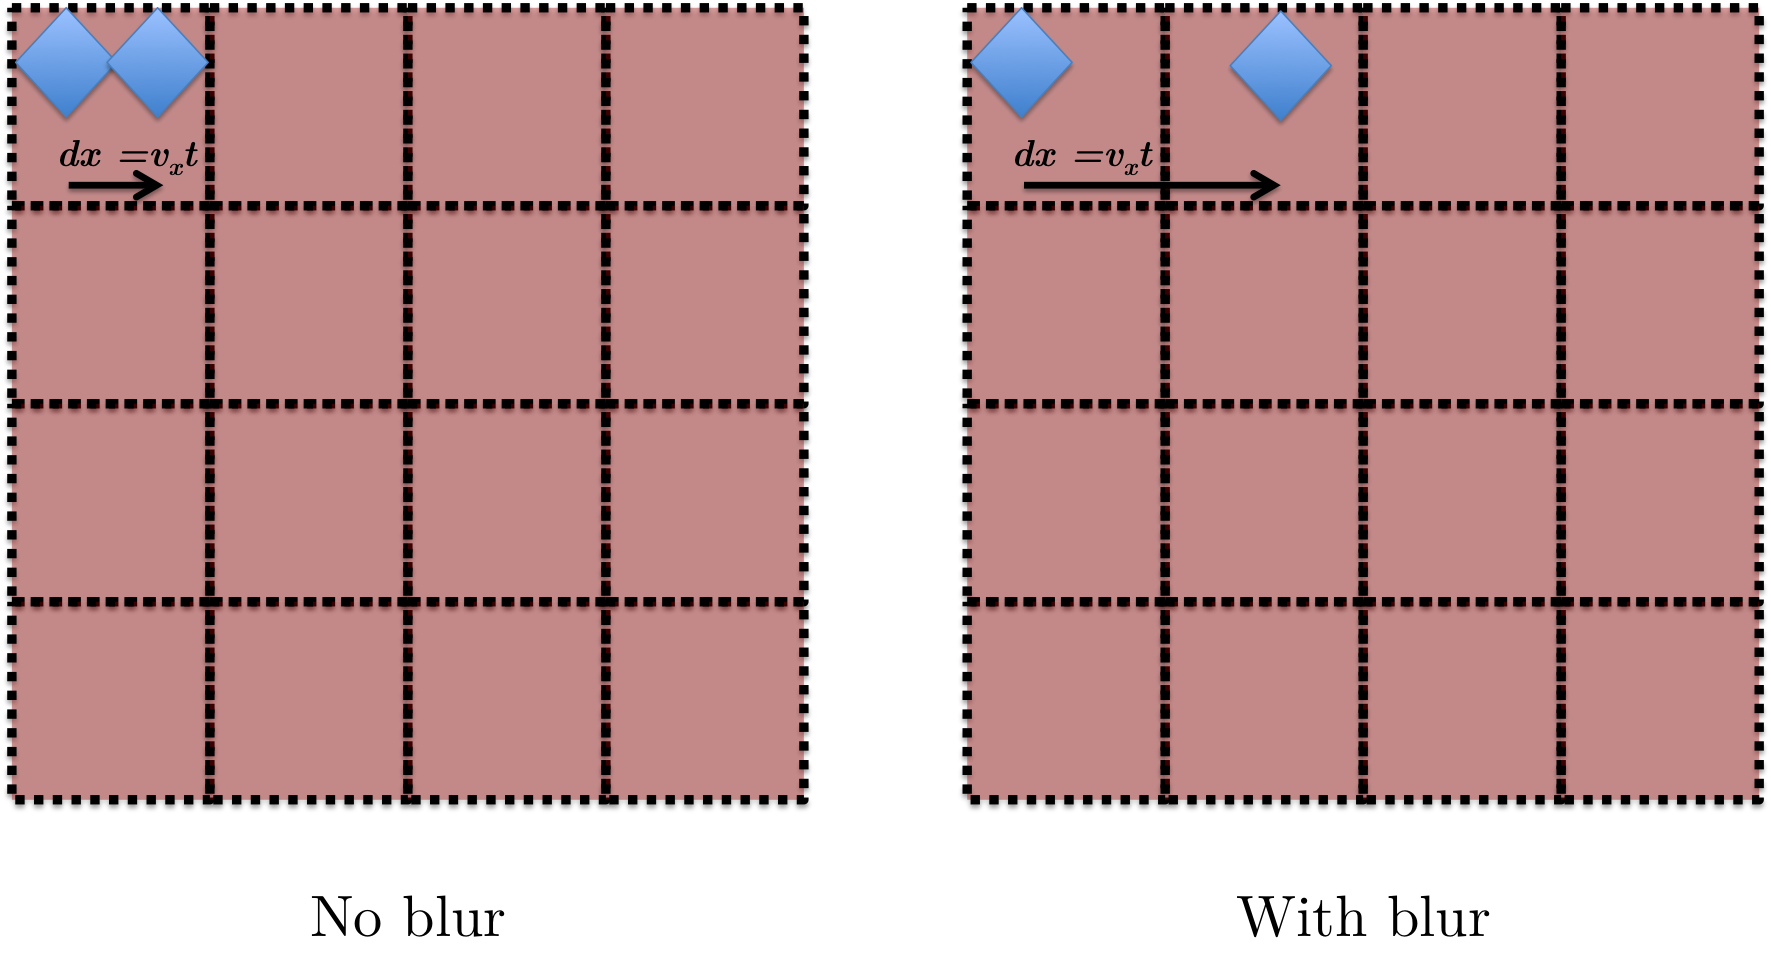
\includegraphics[width=5in]{ccddiagramall}
	\caption{CCD resolution cell diagram, showing cases where an object will be properly resolved and be blurred.}
	\label{fig:ccd}
\end{figure}

\begin{figure}[h!]
\centering
	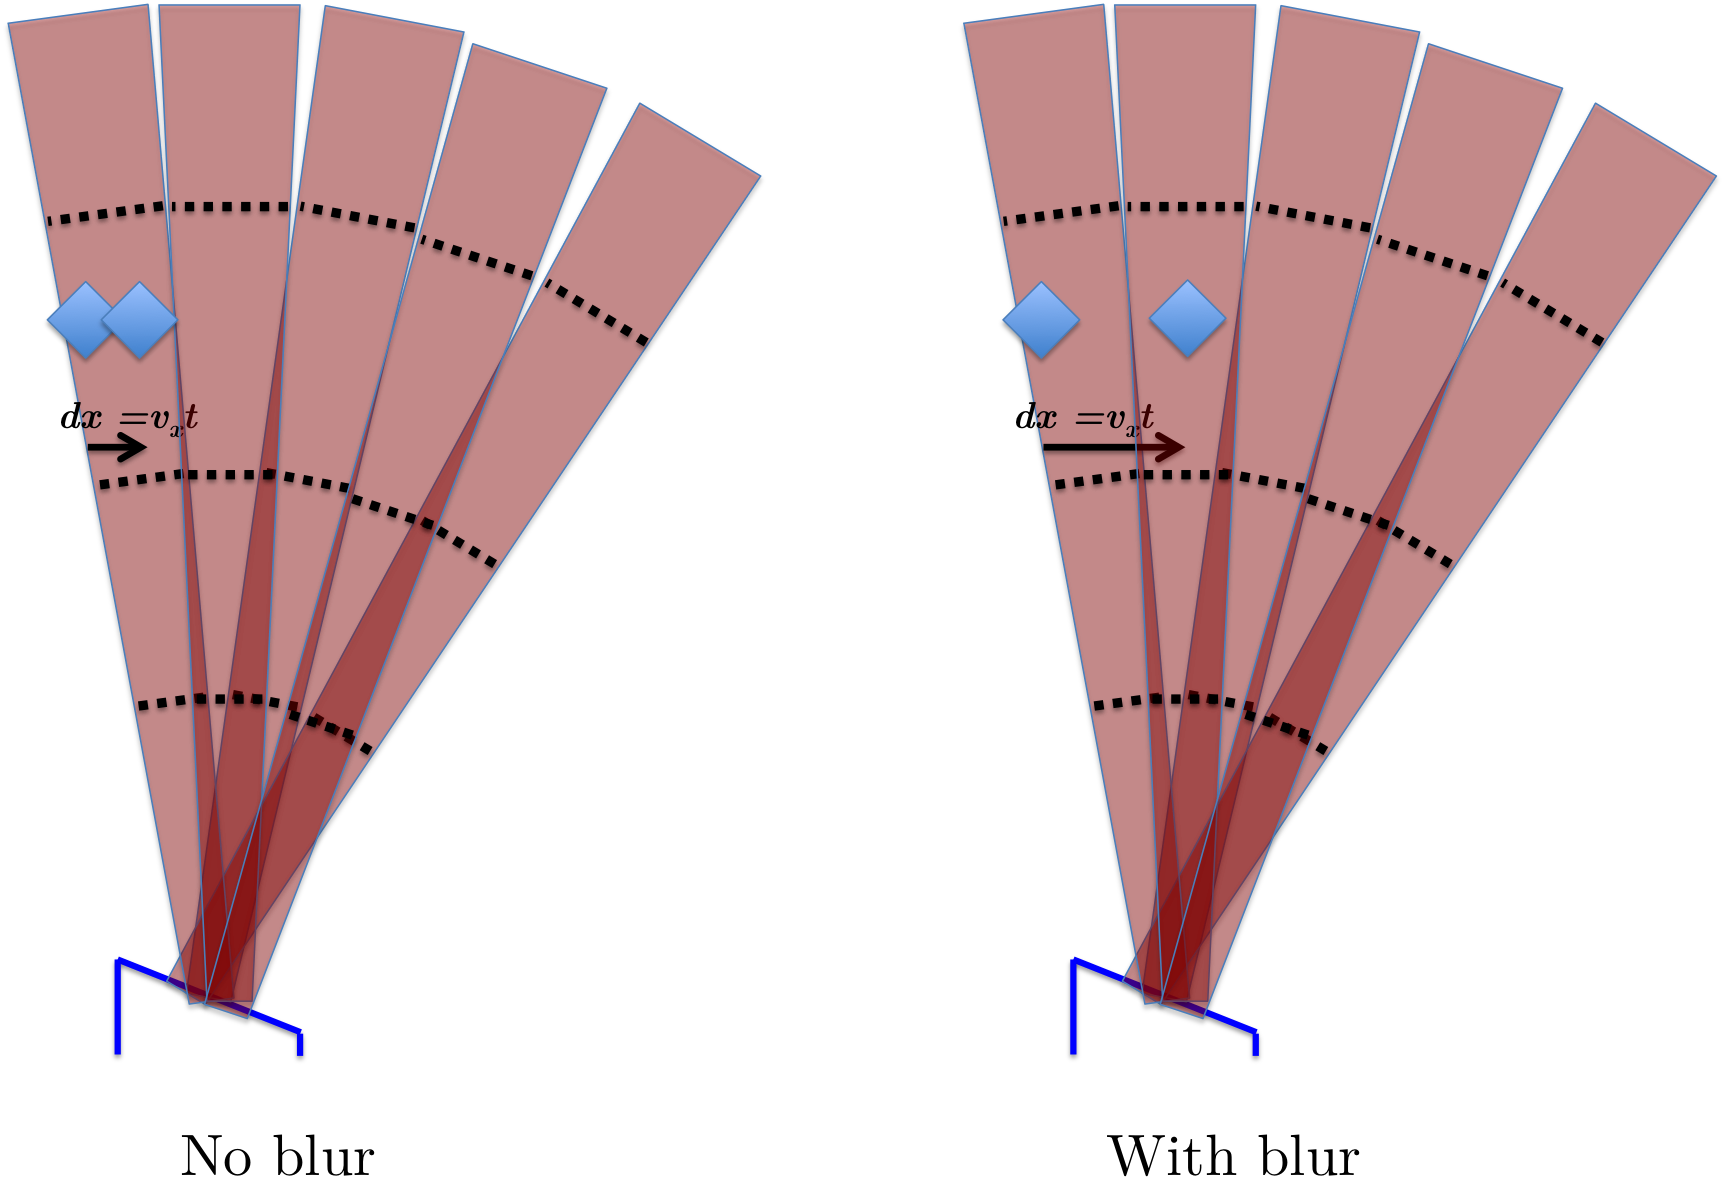
\includegraphics[width=5in]{radardiagramall}
	\caption{ISR resolution cell diagram, showing cases where an object will be properly resolved and be blurred.}
	\label{fig:radarblur}
\end{figure}

\subsubsection{Coordinate System Definitions}

Before the full space-time ambiguity function, $L(\tau_s,\mathbf{r}_s,t_s,\tau,\mathbf{r},t)$, derivation starts the coordinate system will be defined.  The three dimensional coordinate system is defined as $\mathbf{r}=[x,y,z]^T$. For this coordinate system, $\mathbf{r}=[0,0,0]^T$ at the location of the radar and thus $r=|\mathbf{r}|$, also known as the range variable. This allows for the use of polar coordinates $\mathbf{r} =  [r,\theta_,\phi]^T$ where $\theta$ and $\phi$ are, respectively, the observer's elevation and azimuth angles.

The radar samples this space at a set of discrete points which will be referred to as $\mathbf{r}_s = [x_s,y_s,z_s]^T$ along with the discretized range expression $r_s=|\mathbf{r}_s|$. The sampled space consists of a number of points, composed of range gates within a beam multiplied by the number of beams. These points can also be referred in polar coordinates $\mathbf{r}_s = [r_s,\theta_s,\phi_s]^T$, where $\theta_s$  and $\phi_s$ are, respectively, the observationally sampled elevation and azimuth angles.

For notation purposes, two different sets of time are used, commonly known in the hard-target radar literature as fast-time, $n$ and slow-time, $t$ \cite{richards:fundamentalsigproc}. Fast-time is used to describe processes with correlation time less than one PRI. Slow-time will be used for processes that decorrelate in time on the order of, or longer than, the system's PRI. In order to form estimates of ACFs with desired statistical properties, it is assumed that the plasma parameters parameters will change on the order of many tens to hundreds of PRIs in their stationary reference frame (i.e. remain wide sense stationary for this time). Generally, for incoherent scatter applications in the E-region of the ionosphere ($\approx$100 km altitude) and above, the decorrelation time is less than a PRI for systems with a center frequency in the UHF band, and thus ACFs must be formed over fast-time.

The terms $n$ and $t$ represent continuous variables, while $n_s$ and $t_s$ will be the fast time and slow time parameters sampled by the radar. The sampling rate of $n_s$ is set by the rate at which the system's A/D converters are run. The sampling of $t_s$ can, at the highest rate, be the PRI. At its lowest rate, it can be sampled once in a non-coherent processing interval (NCPI), or equivalently in a period of time it takes the radar to average the desired number of pulses for each beam. 

\subsubsection{Derivation}

The physical scattering mechanism underlying ISR produces measurable radar scatter from electron density fluctuations in the ionosphere, $n_e(\mathbf{r},n)$, at a specific wavenumber $\mathbf{k}$. These fluctuations scatter radio waves which can be observed by the receiver system of the radar \cite{dougherty:farley1960}. The emitted radar signal at the transmitter has a pulse shape $s(n)$ modulated at a central frequency creating a scattering wave number $\mathbf{k}$. Using the Born approximation, the signal received at time $n$, $x(n)$, can be represented as the following

\begin{equation}
\label{eq:xt}
x(n) = h(n) \ast \int \exp\left[-j\mathbf{k} \cdot \mathbf{r}\right]  s\left(n-\frac{2r}{c}\right) n_e(\mathbf{r},n) d\mathbf{r},
\end{equation}

\noindent where $h(n)$ is the receiver filter and the $\ast$ represents the convolution operator. In modern ISR systems, this signal $x(n)$ is then sampled at discrete points in fast-time which will be referred to as $n_s$. The convolution and sampling operation can be brought in the integral as the following,

\begin{equation}
\label{ex:xtaug}
x(n_s) = \int \exp\left[-j\mathbf{k} \cdot \mathbf{r}\right]  s\left(n-\frac{2r}{c}\right) n_e(\mathbf{r},n)h(n_s-n) d\mathbf{r}dn
\end{equation}


Once the signal has been received and sampled, the autocorrelation function is then estimated from the sampled signal $x(n_s)$. The full expression of the underlying autocorrelation of this signal is the following, 

\begin{multline}
\label{ex:acf0}
\langle x(n_s)x^*(n_s')\rangle =  \int \exp\left[-j \mathbf{k}\cdot \left(\mathbf{r}'-\mathbf{r} \right)\right]s\left(n-\frac{2r}{c}\right)s^*\left(n'-\frac{2r'}{c}\right) \\ h(n_s-n)h(n_s'-n')\langle n_e(\mathbf{r},n)n^*_e(\mathbf{r}',n')\rangle d\mathbf{r} d\mathbf{r}'dn dn',
\end{multline}

\noindent where $r'$ is the magnitude of the vector $\mathbf{r}'$. By assuming stationarity of second order signal statistics along fast time, lag variables $\tau\equiv n'-n$, and $\tau_s\equiv n_s'-n_s$ can be substituted. With these substitutions, Equation \ref{ex:acf0} becomes


\begin{multline}
\label{ex:acf1}
\langle x(n_s)x^*(n_s+\tau_s)\rangle =\int \exp\left[-j \mathbf{k}\cdot \left(\mathbf{r}'-\mathbf{r} \right)\right]s\left(n-\frac{2r}{c}\right)s^*\left(n+\tau-\frac{2r'}{c}\right) \\ h(n_s-n)h(n_s+\tau_s-n-\tau) \langle n_e(\mathbf{r},n)n^*_e(\mathbf{r}',n+\tau)\rangle d\mathbf{r} d\mathbf{r}' dnd\tau
\end{multline}

\noindent A simplifying assumption at this point that the space-time autocorrelation function of $n_e(\mathbf{r},t)$, $\langle n_e(\mathbf{r},n)n_e(\mathbf{r}',n+\tau)\rangle$, will go to zero as the magnitude of $\mathbf{y} \equiv \mathbf{r}'-\mathbf{r}$ increases beyond the Debye length \cite{farley1969}. Thus, the rate which the spatial autocorrelation goes to zero will be such that $\tau\gg \frac{2||\mathbf{y}||}{c}$, allowing us to set $r= r'$ inside the arguments of $s$ and $h$. This allows Equation \ref{ex:acf1} to be rewritten as 
 
 \begin{multline}
 \label{ex:acf2}
 \langle x(n_s)x^*(n_s+\tau)\rangle = \int s\left(n-\frac{2r}{c}\right)s^*\left(n+\tau -\frac{2r}{c}\right) h(n_s-n)h^*(n_s+\tau_s-n-\tau) \\\left[\int \exp\left[-2j \mathbf{k}\cdot \mathbf{y}\right] \langle n_e(\mathbf{r},n)n^*_e(\mathbf{y}+\mathbf{r},n+\tau)\rangle d\mathbf{y} \right]drdn d\tau.
 \end{multline}

The inner integral is a spatial Fourier transform evaluated at the Bragg vector of radar $\mathbf{k}$. By again asserting stationarity along fast time, the true ACF can be represented as the following,
 \begin{equation}
 \label{eq:spft}
R(\tau,\mathbf{r})= \langle |n_e(\mathbf{k},r,\tau)|^2\rangle \equiv  \int \exp\left[-2j \mathbf{k}\cdot \mathbf{y} \right] \langle n_e(\mathbf{r},b)n^*_e(\mathbf{y}+\mathbf{r},n+\tau)\rangle d\mathbf{y}.
 \end{equation}
 
 \noindent Now Equation \ref{ex:acf2} becomes
 
 \begin{equation}
 \langle x(n_s)x^*(n_s+\tau_s)\rangle = \int \langle |n_e(\tau,\mathbf{k},\mathbf{r})|^2\rangle\left[\int s(n-\frac{2r}{c})s^*(n+\tau -\frac{2r}{c})h(n_s-n)h^*(n_s+\tau_s-n-\tau) dn \right]d\tau dr.
 \end{equation}

 If $n_s$ is replaced with $2r_s/c$ we can introduce the range ambiguity function $W(\tau_s,r_s,\tau,r)$ by doing the following substitution,
 \begin{equation}
 \label{eqn:rngamb}
 W(\tau_s,r_s,\tau,r)= \int s(n-\frac{2r}{c})s^*(n+\tau -\frac{2r}{c})h(2r_s/c-n)h^*(2r_s/c+\tau_s-n-\tau) dn.
 \end{equation}
 
Assuming, for the moment, that $R(\tau,\mathbf{r})$ only varies across the range dimension $r$, this can be represented in the form of a Fredholm integral equation
 
 \begin{equation}
 \label{eqn:fredfirst}
 \langle x(2r_s/c)x^*(2r_s/c+\tau_s)\rangle = \int W(\tau_s,r_s,\tau,r)R(\tau,r) drd\tau.
 \end{equation}
 
\noindent The range ambiguity function, $W(\tau_s,r_s,\tau,r)$, can be thought of as a smoothing operator along the range and lag dimensions of $R(\tau,r)$. This result is also derived in \cite{nikoukar2008}, \cite{Woodman:1991is} and \cite{hysell2008}

 
The spatial ambiguity across azimuth and elevation angles is determined by the antenna beam pattern. In phased array antennas, this beam pattern is ideally the array factor multiplied by the element pattern \cite{Balanis:2005:ATA:1208379}. The array factor is determined by a number of things including the element spacing and the wave number of the radar, $k$. For example, by making idealized assumptions with no mutual coupling and that the array elements are simple cross dipole elements, AMISR systems will have the following antenna pattern for pointing angle ($\theta_s,\phi_s$): 

 \begin{equation}
 \label{eqn:amisrpat}
F(\theta_s,\phi_s,\theta,\phi) = \frac{1}{2}(1+\cos(\theta)^2)\left[ \frac{1}{MN} \left(1+\exp\left[j(\psi_y/2 + \psi_x)\right]\right)\frac{\sin((M/2) \psi_x)}{\sin(\psi_x)} \frac{\sin((N/2) \psi_x)}{\sin(\psi_x/2)}\right]^2,
 \end{equation}
 
 \noindent where $\psi_x = -k d_x(\sin\theta\cos\phi-\sin\theta_s\cos\phi_s)$, $\psi_y = -k d_y(\sin\theta\sin\phi-\sin\theta_s\sin\phi_s)$ and $M$ is the number of elements in the $x$ direction of the array, and $N$ is the number of elements in the $y$ direction(see Appendix: \ref{App:AMISRarr} for derivation).


The spatial ambiguity is a separable function made up of the components of $W(\tau_s,\tau,r_s,r)$ and $F(\theta_s,\phi_s,\theta,\phi)$. These two functions can be combined by multiplying the two, creating the spatial ambiguity function  $K(\tau_s,\mathbf{r}_s,\tau,\mathbf{r})$. This yields an expression for a single statistical realization of the ACF of the incoherent scatter random process, which will be referred to as $\rho(\tau_s,\mathbf{r}_s)$:


 \begin{align}
  \label{eqn:volume}
\rho(\tau_s,\mathbf{r}_s) &= \int F(\theta_s,\phi_s,\theta,\phi)W(\tau_s,r_s,\tau,r) R(\tau,\mathbf{r}) dV d\tau ,\\
	&= \int K(\tau_s,\mathbf{r}_s,\tau,\mathbf{r}) R(\tau,\mathbf{r})  dVd\tau.
\end{align}

A rendering of an example of this full spatial ambiguity function for an uncoded long pulse, with antenna pattern from Equation \ref{eqn:amisrpat} for four beams, can be seen in Figure \ref{fig:amb4}.

\begin{figure}
	\centering
	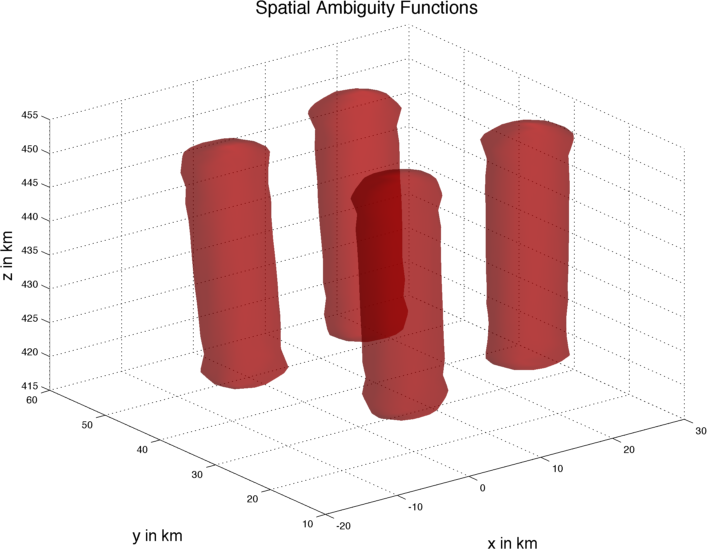
\includegraphics[width=4in]{spaceamb}
	\caption{Full spatial ambiguity function in Cartesian space for case with 4 beams with trailing edge of a 240$\mu$s pulse at 400km range. The surface represents the half power point of the ambiguity function.}	
	\label{fig:amb4}
\end{figure}

As mentioned above, this one pulse ACF estimate represents a single sample of a random process. In order to create a usable estimate, multiple samples of this ACF need to be averaged together to reduce the variance to sufficient levels in order to fit the estimate to a theoretical ACF that is a direct function of plasma parameter values. To show the impact of this averaging in creating the estimate of the ACF, a slow-time dependence will be added to the expression for the medium ACF, which now becomes $R(\tau,\mathbf{r},t)$, and will also add another separable function $G(t_s,t)$ to the kernel. This function $G(t_s,t)$ can be thought of as a sampling and blurring kernel for the ACF if the plasma parameters change within an NCPI. Since the amount of time that the radar pulse is illuminating the plasma in a point of space is very short compared to the PRI, $G(t_s,t)$ can take the form of a summation of Dirac delta functions 

\begin{equation}
\label{eqn:Gexp}
G(t_s,t) = \displaystyle \sum_{j=0}^{J-1}\alpha_j \delta(t-t_s-jT_{REV}),
\end{equation}

\noindent where $J$ counts the number of pulses used over a NCPI, $T_{REV}$ is the amount of time it takes the radar to revisit the specific beam and $\alpha_j$ represent the weights that the radar assigns to the pulses. For systems using pulse-to-pulse steering, one strategy revisits each beam sequentially, in this case making $T_{REV}=N_{beam}T_{PRI}$, where $N_{beam}$ is the number of beams and $T_{PRI}$ is the PRI time period. For the case where weights are set to $1/J$, this operation simply averages the pulses. With Equation \ref{eqn:Gexp} incorporated into the overall ambiguity we obtain the full integral equation,

\begin{equation}
\label{eqn:sptamb}
	\rho(\tau_s,\mathbf{r}_s,t_s) =\int L(\tau_s,\mathbf{r}_s,t_s,\tau,\mathbf{r},t)R(\tau,\mathbf{r},t)dVdtd\tau.
\end{equation}

\noindent The final kernel, $L(\tau_s,\mathbf{r}_s,t_s,\tau,\mathbf{r},t) = G(t_s,t)K(\tau_s,\mathbf{r}_s,\tau,\mathbf{r})$, encompasses the full space-time ambiguity.

\section{Ambiguity after Frame Transformation}
\label{sec:frametrans}

This section will focus on the impact of the motion of plasma as it is going through the field of view of the radar. It will be assumed that the radar is integrating over a length of time $T$ beginning at $t_s$. The kernel $L$ will be represented as a separable function $K$ and $G$ as in Equation \ref{eqn:sptamb}. In this case, $G$ will be a summation of Dirac delta functions with weights of $1/J$. This will change Equation \ref{eqn:sptamb} to the following:

\begin{equation}
\label{eqn:L2}
\rho(\tau_s,\mathbf{r}_s,t_s) = \int K(\tau_s,\mathbf{r}_s,\tau,\mathbf{r}) \left[(1/J)\int_{t_s}^{t_s+T} \displaystyle \sum_{j=0}^{J-1} \delta(t-t_s-jT_{REV})R(\tau,\mathbf{r},t) dt\right] dVd\tau.
\end{equation}

Of specific interest in this study are instances in the high latitude ionosphere where embedded plasma structures are moving due to electric field drivers applied by the magnetosphere. In this case, it will be assumed that the plasma is a rigid object and will not deform with respect to $\mathbf{r}$ over time period $[t_0,t_0+T]$ where $T=JT_{REV}$ is the time for one NCPI. Also, it will be assumed that the plasma parcel moves with a constant velocity $\mathbf{v}$. Thus $R(\tau,\mathbf{r},t)\Rightarrow R(\tau,\mathbf{r}+\mathbf{v}t)$. The assumption of rigidity can in some cases be valid over the time period of the NCPI, on the order of a few minutes, while the plasma moves through the field of view of the radar. For example, in the high latitude ionosphere, large scale features in structures such as patches decay on the order of hours \cite{Tsunoda:1988ul}. This assumption is useful because it allows our framework to analyze impacts of these plasma variations on the parameter resolution of ISR systems. With these assumptions, Equation \ref{eqn:L2} becomes,

\begin{equation}
\label{eqn:L3}
\rho(\tau_s,\mathbf{r}_s,t_s) =(1/J) \int \int_{t_s}^{t_s+T} \displaystyle \sum_{j=0}^{J-1}\delta(t-t_s-jT_{REV}) K(\tau_s,\mathbf{r}_s,\tau,\mathbf{r})R(\tau,\mathbf{r}+\mathbf{v}t)dtdVd\tau\end{equation}

A change of variables to $\mathbf{r}' = \mathbf{r}+\mathbf{v}t$ acts as a Galilean transform and applies a warping to the kernel, changing the frame of reference. Since $R(\tau,\mathbf{r}')$ is no longer dependent on $t$, Equation \ref{eqn:L3} can be integrated in time and becomes:

\begin{equation}
\label{eqn:L5}
\rho(\tau_s,\mathbf{r}_s,t_s)= (1/J)\int \left[ \;\;  \displaystyle \sum_{j=0}^{J-1} K(\tau_s,\mathbf{r}_s,\tau,\mathbf{r}'-\mathbf{v}(t_s+jT_{REV})) \;\; \right]R(\tau,\mathbf{r}')dVd\tau.
\end{equation}

The problem can now be simplified further back to a Fredholm integral equation by simply replacing the terms in the square brackets as a new kernel $A(\tau_s,\mathbf{r}_s,t_s,\tau,\mathbf{r}')$:

\begin{equation}
\label{eqn:L6}
\rho(\tau_s,\mathbf{r}_s,t_s)= \int A(\tau_s,\mathbf{r}_s,t_s,\tau,\mathbf{r}') R(\tau,\mathbf{r}')dVd\tau.
\end{equation}

\noindent The impact of the plasma velocity on the ambiguity function can be seen in Figure \ref{fig:ambtime}. This is the same ambiguity as seen in Figure \ref{fig:amb4} but with a velocity of 500 m/s in the $y$ direction over a period of 2 minutes. This velocity creates a larger ambiguity function in the frame of reference of the moving plasma.

\begin{figure}[!t]
	\centering
	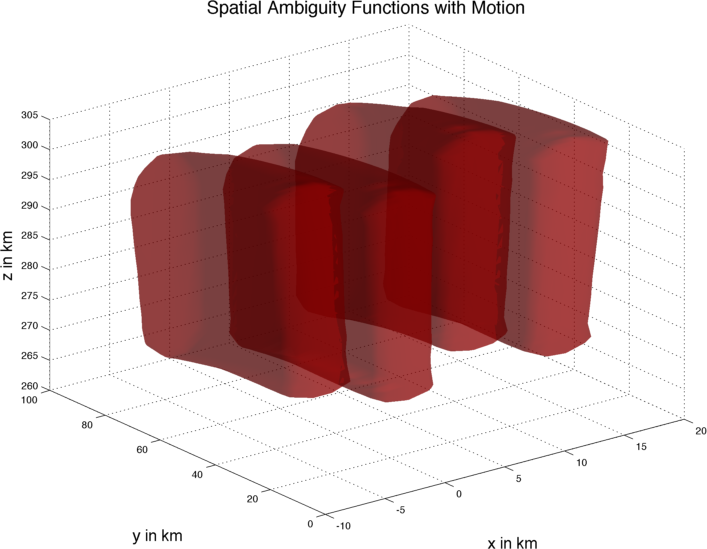
\includegraphics[width=4in]{spaceambmoving}
	\caption{Same spatial ambiguity as in Figure \ref{fig:amb4} but now with 500 m/s velocity in $y$ direction in plasma frame of reference. The surface represents the half power point of the ambiguity function.}
	\label{fig:ambtime}
\end{figure}

The operator $A$ can be determined through knowledge of the radar system's beam pattern along with the experiment's pulse pattern, integration time and inherent velocity of the plasma. This velocity $\mathbf{v}$ could be separately estimated by taking measurements of the Doppler shift by using a methodology like that seen in \cite{butler:imagingfregiondrifts}. With this strategy, the operator is now acting purely as a spatial blurring function instead of a full space-time function. It is noted that reducing dimensionality of the problem can make it easier to solve the inverse problem in practice.

\section{Example of Impact on Real ISR Data}

With knowledge of the ambiguity the possible size of features can be inferred. An example using real data can further elucidate this idea. One way that the true size of features is comparing real data with possible inputs and applying the ambiguity to them. Often, researchers using ISR combine data from different sensors \cite{Dahlgren:2012dq}, such as all sky camera data \cite{Shiokawa1999,GRL:GRL21871,Shiokawa2009}. This allows for researchers to get a better understanding of the underlying physical phenomena.

An example of real data that shows how features could have been impacted by this ambiguity is seen through the series of images in Figure \ref{fig:realdataplane3points}. The auroral arc, seen as an electron density enhancement in the radar data and a brightness enhancement in the optical data, is moving along horizontal position of the plane over a two minute integration period for each image. The radar data is sampled in a spherical coordinate space, thus it is necessary to use some sort of interpolation to view it on the plane of motion, in this case natural neighbors. 

\begin{figure}[h!]
	\centering
	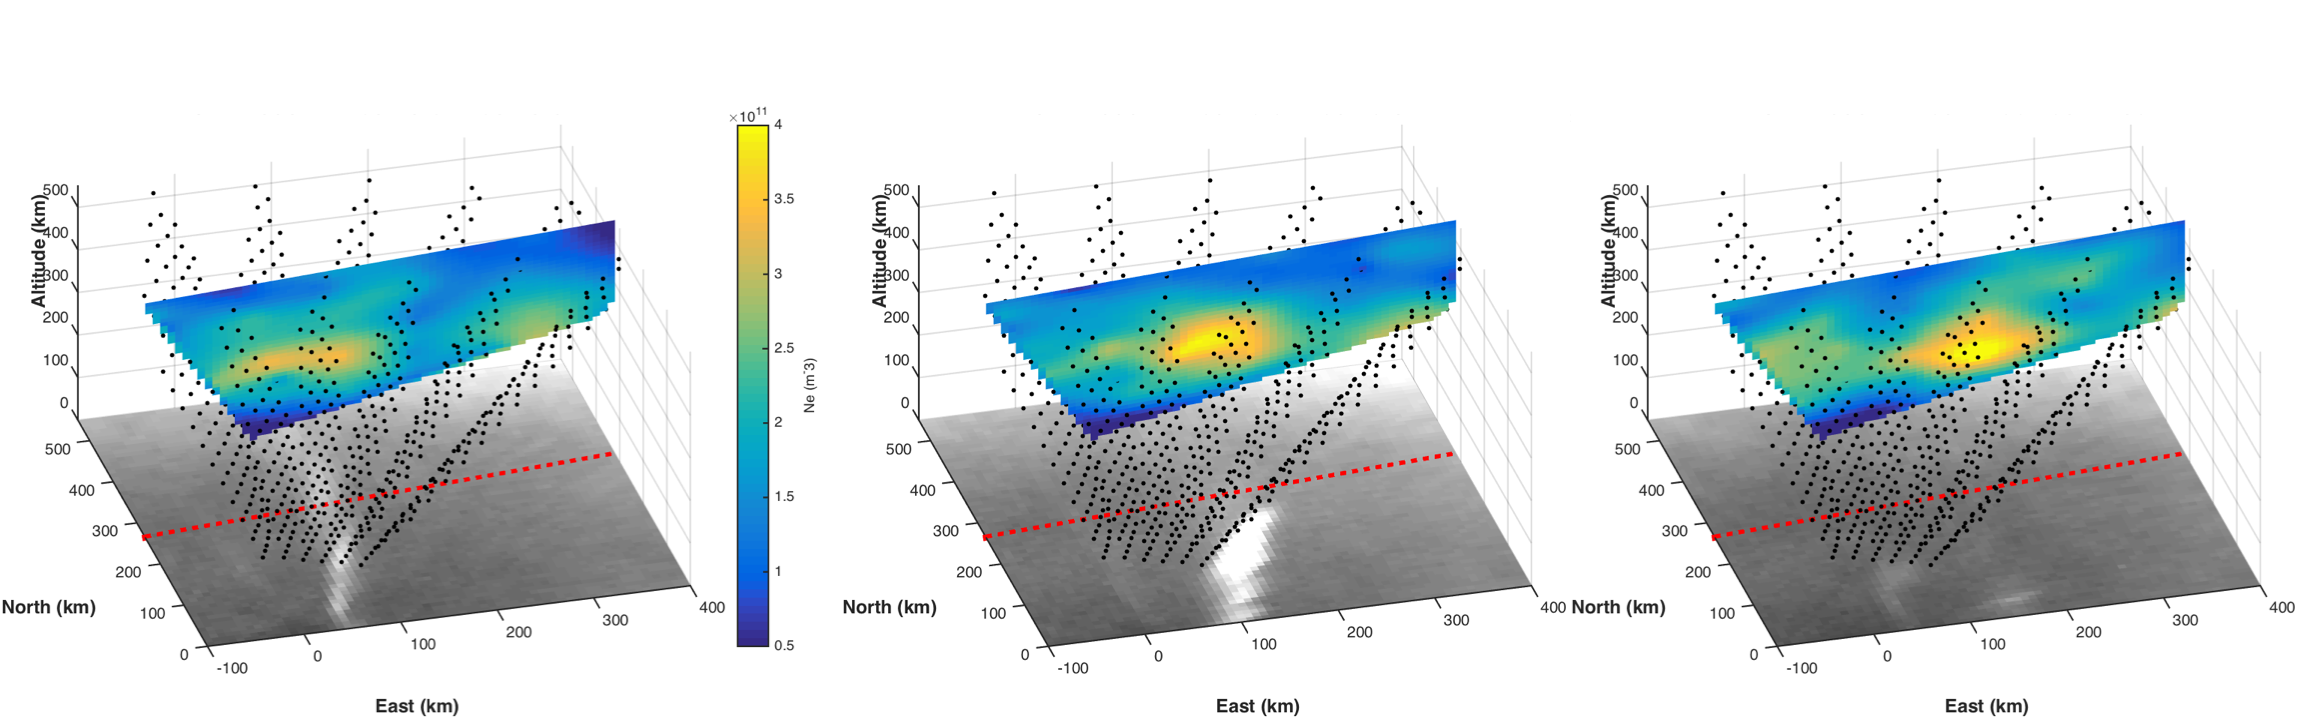
\includegraphics[width=6in]{radarwithoptical}
	\caption{Data taken from the Resolute Bay Incoherent Scatter Radar (RISR) and interpolated along the plane of motion of the auroral arc with green line emission optical data plotted underneath. Each image is a plotted over a two minute integration time for the radar. Also in the image is the sample points of the radar (black dots) and the path of the auroral emission. }
	\label{fig:realdataplane3points}
\end{figure}

The final set of radar data seen in Figure \ref{fig:realdataplane3points} is replotted in Figure \ref{fig:realdataplane} without other data sets and sampling grids. This will help with the comparisons to the following figures, which are plotted along the same plane of motion.

\begin{figure}[h!]
	\centering
	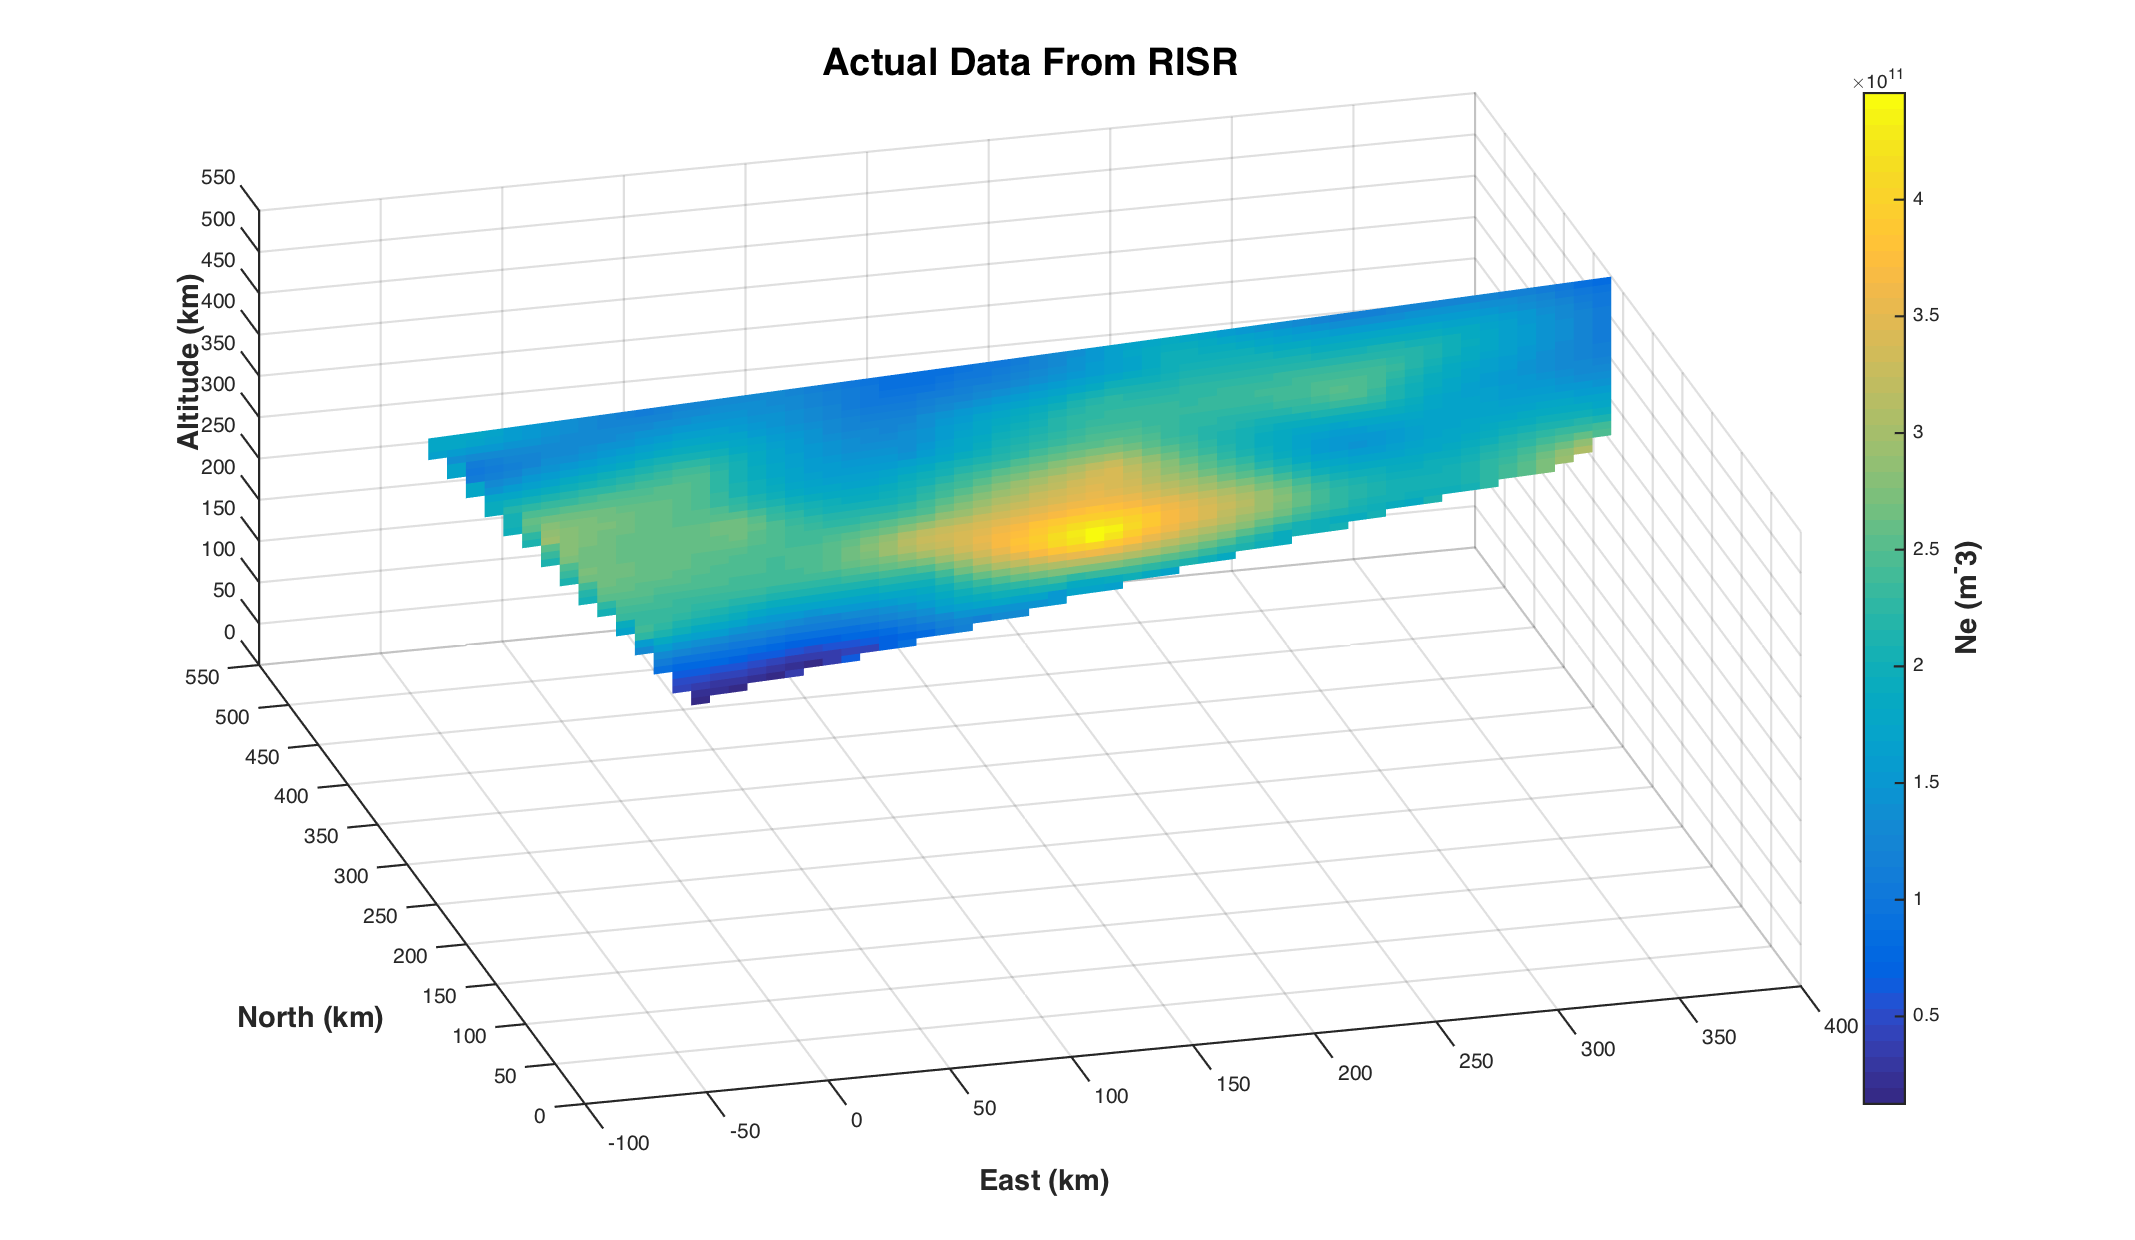
\includegraphics[width=4in]{acdata}
	\caption{Data taken from the Resolute Bay Incoherent Scatter Radar (RISR) and interpolated along the plane of motion of the auroral arc.}
	\label{fig:realdataplane}
\end{figure}

The specific experiment beam pattern yielded a sampling pattern seen as the black dots in \ref{fig:rambplane}. The specific result of the ambiguity along the the plane of the motion can give a basic idea of the "resolution" of the image of the objects if there is not motion. Also it can show if an object may be hidden if stationary during the integration time.

\begin{figure}[h!]
	\centering
	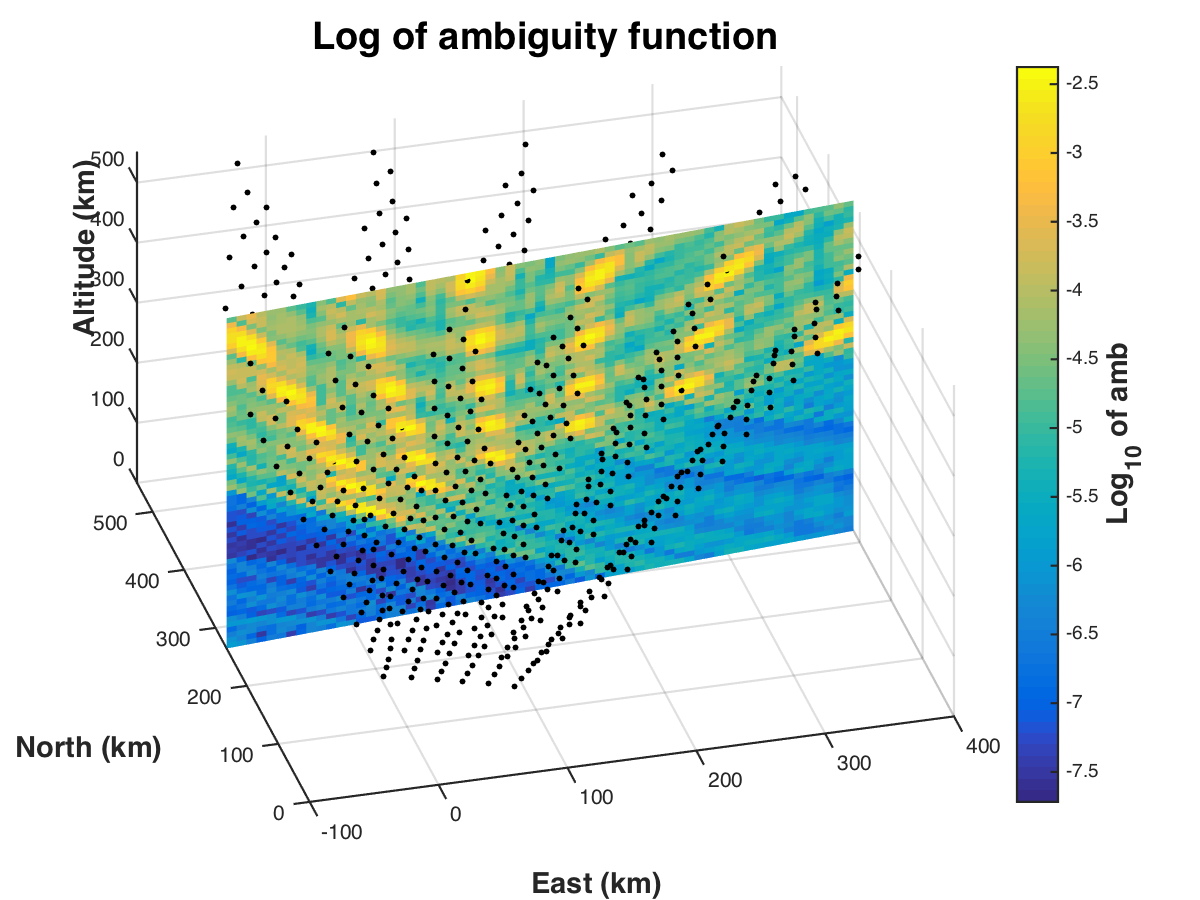
\includegraphics[width=4in]{ambplane}
	\caption{The three dimensional sampling pattern as black dots and spatial ambiguity plotted on to along the plane of motion along the auroral arc.}
	\label{fig:rambplane}
\end{figure}

In order to find the actual size of the feature in Figure \ref{fig:realdataplane} we have to take into account the ambiguity in Figure \ref{fig:rambplane} along with any motion that may be present in the feature. The feature shown in Figure \ref{fig:simdataplaneorig} is a possible distribution that could create a similar measurement seen in Figure  \ref{fig:realdataplane}. Using the optical data we have inferred that that this feature is from a cylinder with a Gaussian shaped cross-sectional plasma density. 

\begin{figure}[h!]
	\centering
	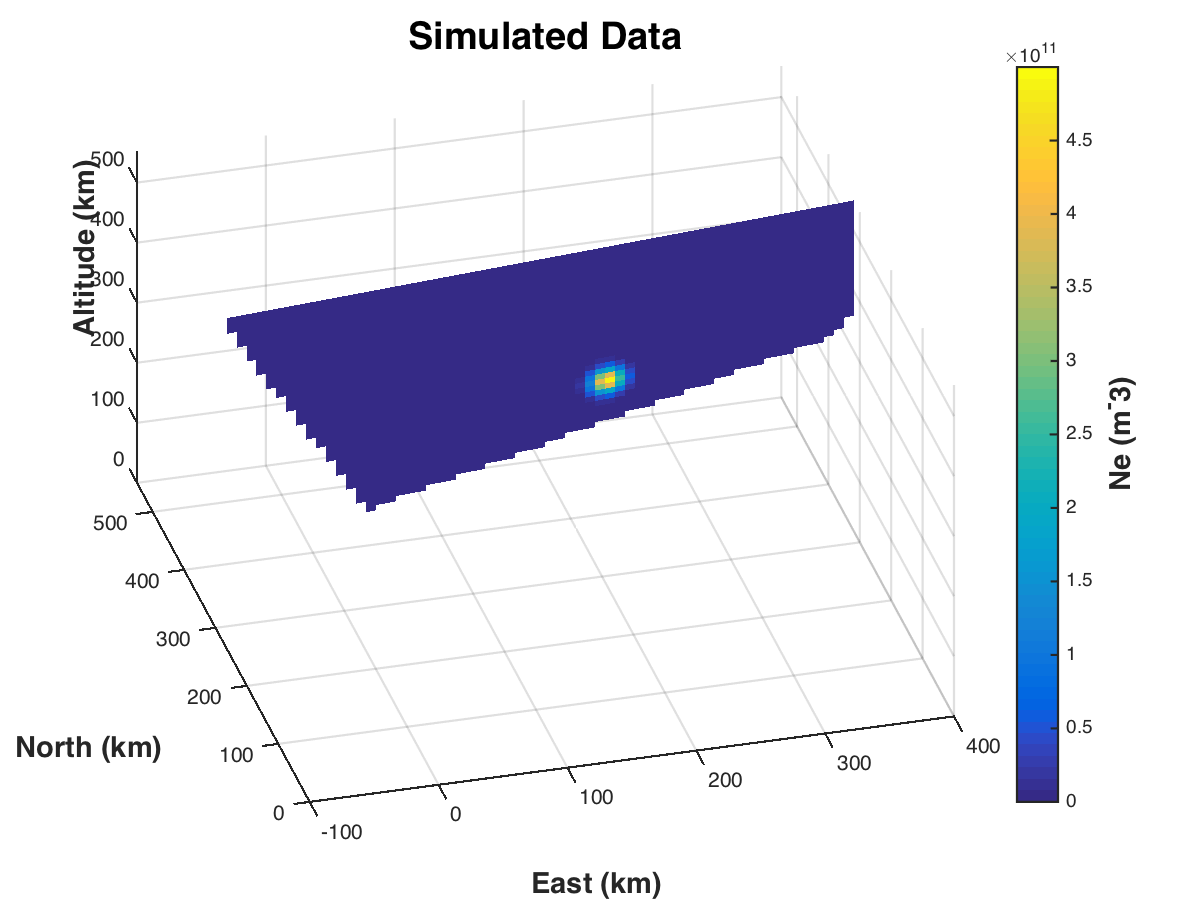
\includegraphics[width=4in]{simdataplaneorig}
	\caption{A possible distribution of electron density with a Gaussian shaped enhancement that has a max of 5x10$^{11}$ m$^{-3}$  a standard deviations of 12.7 km along the vertical direction and 8.5 km along the horizontal direction. The center of this plotted at the point $\mathbf{r}=[ 225\text{km}, 225 \text{km},335\text{km}]^T$. It is assumed that the density is constant along the direction orthogonal to the plane of motion.}
	\label{fig:simdataplaneorig}
\end{figure}

Applying the space time ambiguity in Figure \ref{fig:rambplane} along with an assumed motion of 500 m/s, which again suggested by the data in Figure \ref{fig:realdataplane3points}, the distribution in Figure \ref{fig:simdataplane} is created. This seems to suggest that the features seen in Figure \ref{fig:realdataplane} could be from physical phenomena that is much smaller than what is shown in the interpolated image. 

\begin{figure}[h!]
	\centering
	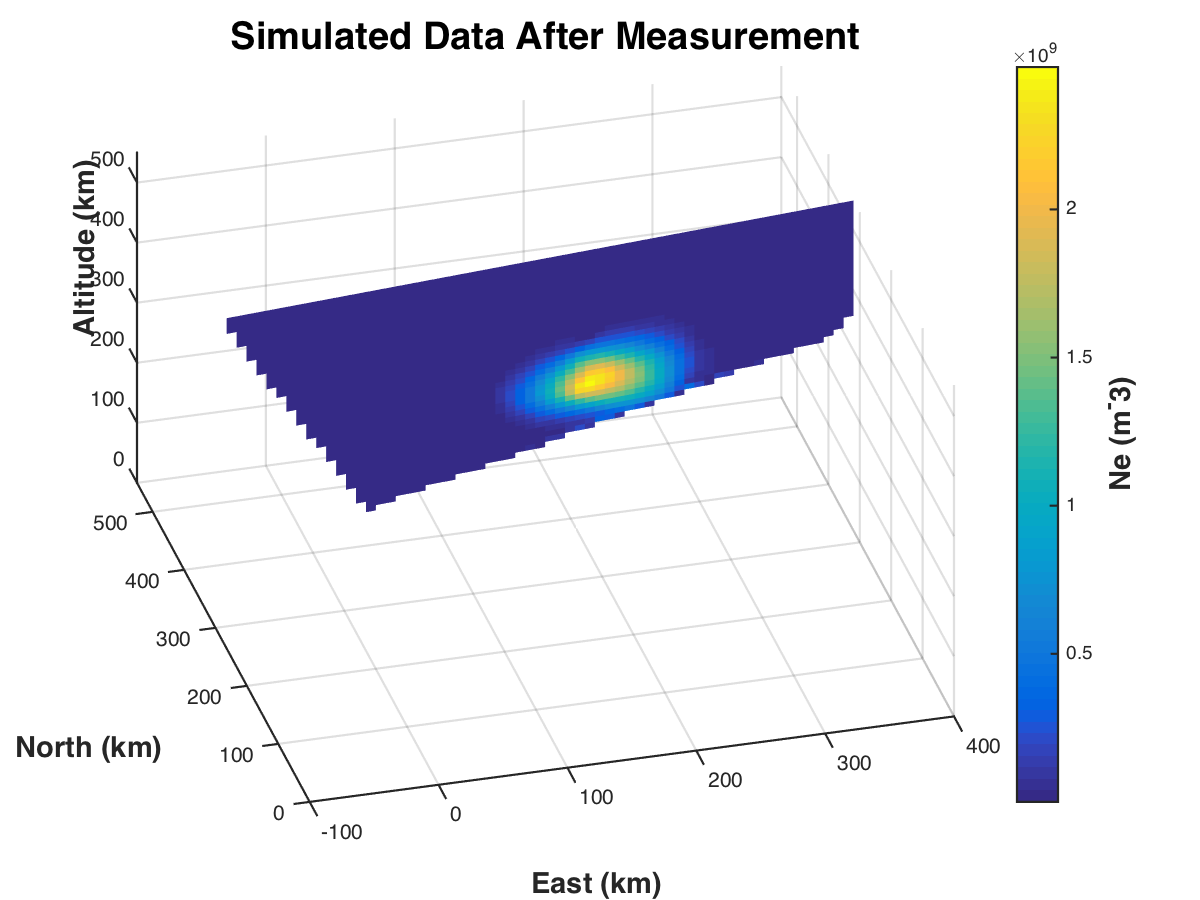
\includegraphics[width=4in]{simdataplane}
	\caption{The same feature from Figure \ref{fig:simdataplaneorig} after applying the effect the spatial ambiguity seen in \ref{fig:rambplane} and 500 m/s motion over the two minute integration period.}
	\label{fig:simdataplane}
\end{figure}

\section{Discussion}

The use of the Space-Time Ambiguity function as a kernel of Fridholm integral equation is the theoretical framework of this thesis. The process for the estimation of the ACFs fits very well within this mathematical structure. This structure though, is not rigid and can be adapted to the situation that a researcher may face when performing ISR experiments by taking advantage of the fact that the ambiguity kernel is a set of separable functions. The ambiguity can be used similar as a blurring kernel if there is plasma motion which can allow one to set of different possible features, thus creating an ill-posed inverse problem. Lastly, this can easily be demonstrated in experiments where real data is used.